 \section{Introduction}
\label{sec:intro}
% Introduce the concept of Social Deduction Games and why playing them with BDI agents and LLMs is an interesting challenge. Outline the structure of the report.
\subsection{Modified Set of Rules}
\label{subsec:modifiedRules}

While the original rules of the game are documented in \cite{mafia_wiki}, several structural modifications were implemented in this project. 
These changes are designed to enhance the realism of the game, accommodate the erratic behavior of the agents, and improve the user experience for human players:

\begin{itemize}
    \item \textbf{Flexible Role Assignment:} The traditional recommendation of a 1:3 ratio between Werewolves and Villagers is not strictly enforced; the game can be initialized with any arbitrary numerical distribution of roles by simply defining a custom set of players and roles within the \texttt{werewolf.jcm} file.
    
    \item \textbf{Nocturnal Hunt Mechanics:} During the night phase, Wolves select a victim using a \emph{plurality vote} (the highest vote count wins). To simulate realistic behavior (e.g. players that does not really understand the goal of the game), Wolves are allowed to vote for other Wolves. Since text communication is disabled at night, they are granted up to \textbf{3 consecutive voting rounds}\footnote{This allows the wolves to to silently coordinate by observing each other's previous votes; else they have no way to align themselves, since the only phase with explicit communication is the public Discussion Phase.}. If a tie remains after the third round, the hunt fails and no player is eliminated.
    
    \item \textbf{Structured Discussion Phase:} The daytime discussion is strictly limited to an exchange of exactly  \textbf{7 messages}. The floor is granted to players who explicitly request to speak, resolved through a strict priority hierarchy (Subsection \ref{subsubsec:speaker_selection}).

    
    \item \textbf{Daytime Execution Vote:} The village execution vote consists of a single voting round utilizing the same plurality system as the nocturnal hunt. In the event of a tie, no execution takes place and the game proceeds to the next night phase.
    
    \item \textbf{Terminal Conditions:} The game only concludes upon the total annihilation of one faction: either all Wolves are eliminated, or all Villagers are eliminated. This intentionally deviates from the standard rule where Wolves win automatically upon reaching numerical parity with the Villagers\footnote{This change allows for edge cases where a dominant Wolf pack might still lose the game due to erratic internal voting or self-sabotage.}.
\end{itemize}

\subsection{Overview of the Project}
\label{subsec:overview}

The in-depth explanation of the project's functionalities follows a layered approach, starting from the most bare-bones version of the system, consisting solely of the core game engine driven by the \textbf{Narrator} (Section \ref{sec:narrator}) and the purely symbolic \textbf{players} (Section \ref{sec:players}). 

\begin{figure}[H]
    \centering
    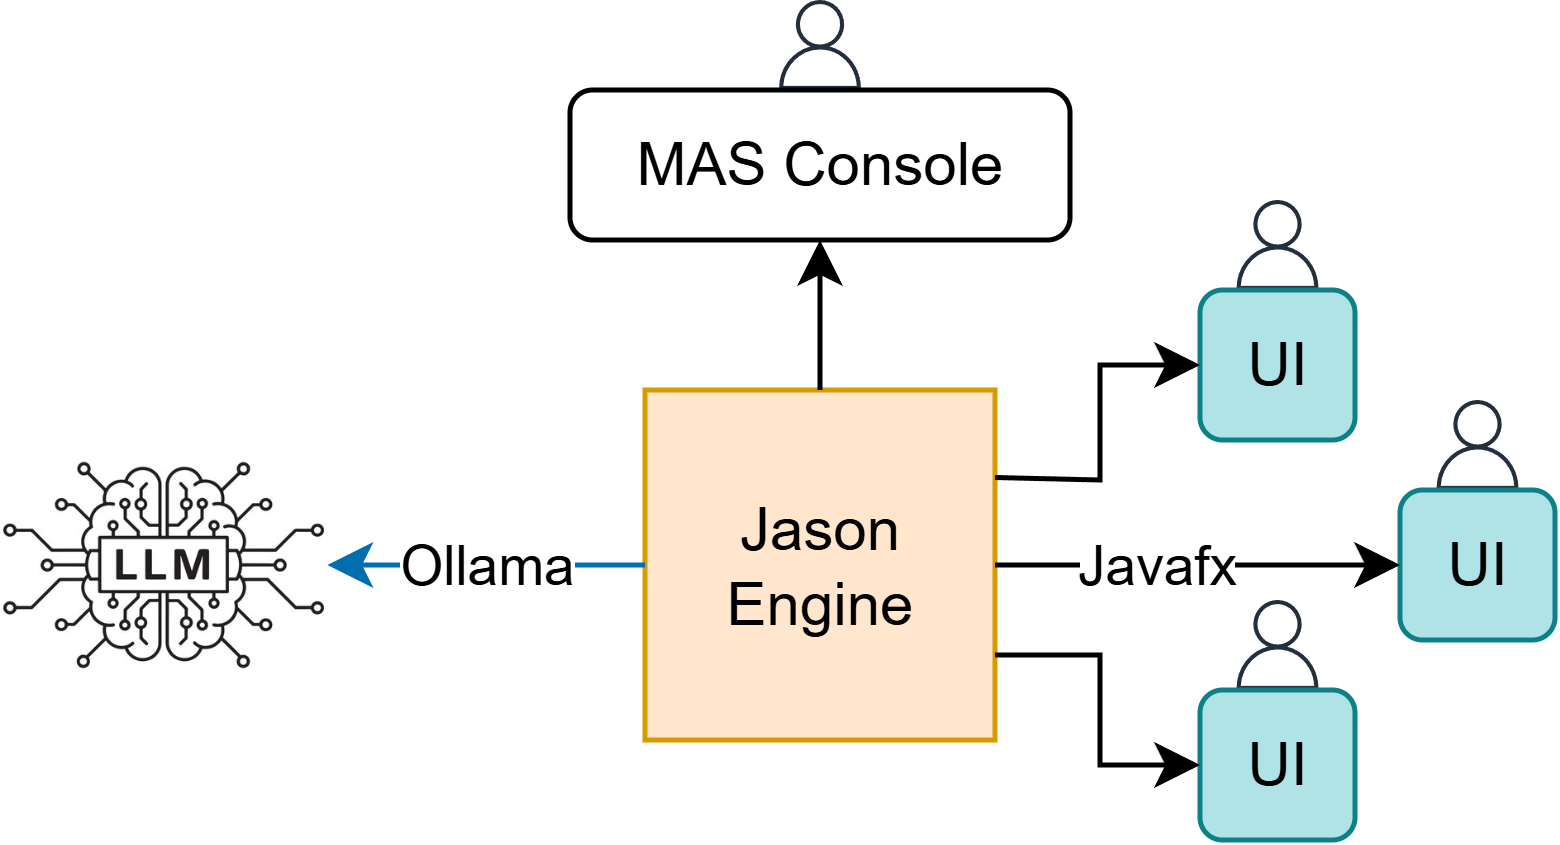
\includegraphics[width=0.8\textwidth]{images/schema.png}
    \caption{High-level schematic of the project modules: the Jason engine acts as the bare-bone central orchestrator, Ollama provides LLM capabilities, and JavaFX drives the User Interfaces.}
    \label{fig:architecture_schema}
\end{figure}

Building upon this standalone symbolic core, we subsequently introduce the \textbf{JavaFX User Interface} (Section \ref{sec:ui}) to enable human-driven player interactions and spectator observability. Finally, we detail the custom \textbf{Ollama API} (Section \ref{sec:llm}), which is integrated into the architecture to facilitate both Natural Language Generation (NLG) and reasoning for LLM-driven autonomous players.